\chapter{Popis navržených řešení}

V předešlé kapitole byla vysvětlena základní problematika, která souvisí s virtualizací síťových funkcí, cloud computingem a softwarově definovanými sítěmi. Zároveň byla popsána referenční architektura frameworku pro virtualizaci síťových funkcí. Tato kapitola bude již věnována konkrétnímu příkladu využití virtuálních síťových funkcí v cloudovém prostředí. Nejprve zde popsána navržená architektura pro privátní cloudovou platformu využívající virtualizaci síťových funkcí, kterou mohou využívat všichni její uživatelé. Pro tuto cloudovou platformu a pro její uživatele byli navrženy dva příklady virtuálních síťových funkcí. U obou příkladů jsou uvedeny scénáře a způsob jakým jsou navrženy.

\section{Požadavky na VNF řešení}

\begin{itemize}
\item Univerzálnost - Celé řešení musí být postavené tak, aby ho mohli využívat všichni uživatelé dané cloudové platformy. 
\item Jednoduchost - 
\item Otevřenost a Flexibilita - 
\item Kompatibilita se stávající síťovými prvky - 
\end{itemize}

\section{Architektura navrženého řešení}

Architektura navrženého řešení byla implementována pomocí cloudové platformy OpenStack a SDN řešení OpenContrail. Obrázku č. \ref{fig:VNF_overview} znázorňuje tyto technologie v souvislosti s referenční architekturou popsanou v kapitole \ref{sub:architektura}. Je nutné říci, že obě technologie nezapadají přímo do jedné z částí referenční architektury. Naopak v některých případech se překrývají nebo se v ní doplňují.

\begin{figure}[h]
\begin{centering}
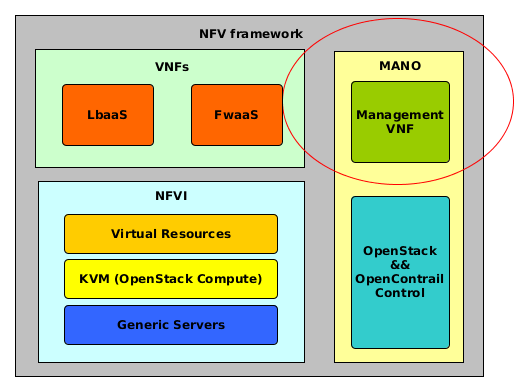
\includegraphics[scale=0.51]{images/VNF_overview}
\par\end{centering}
\caption{Architektura NFV řešení\label{fig:VNF_overview}}
\end{figure}

OpenStack byl zvolen, protože se jedná o největší open-source cloudovou platformu na světě. OpenStack tvoří část správy infrastruktury. Hardwarová vrstva infrastruktury se může skládat z libovolných serverů, na kterých je nainstalován KVM hypervizor. Tento hypervizor tvoří virtuální vrsvu a byl vybrán, protože je nejčastěji používán společně s OpenStackem. Avšak v případě potřeby by zde mohl být použit i jiný hypervizor, pokud bude zachována kompatibilita vůči OpenStacku.

OpenStack spravuje převážně zdroje týkající se výpočeního výkonu (Compute) a uložiště (Storage). Tyto zdroje následně přiděluje dle potřeby virtuálním instancím nebo v našem případě instancím, které slouží jako VNF.

Speciálně pro vyřešení síťování v této infrastruktuře je součástí řešení OpenContrail. Díky tomu je možné vytvářet overlay sítě pomocí VXLAN či MPLSoverGRE, kterými jsou dynamicky propojovány jednotlivé VM a VNF. 

Jednotlivá VNF mohou být v OpenContrailu vytvořena pomocí tzv. Servisních Instance a Servisní Templatů. Ty budou v této práci použity pro vytvoření VNF sloužící jako Firewall a budou podrobně popsány v kapitole věnující se vytváření této služby.

Další součástí, která musela být v architektuře navrhnuta, je způsob řízení a správy jednotlivých VNF. Zde se muselo jednat o řešení, jakým automaticky vytvořit a popřípadě i smazat všechny potřebné části potřebné pro VNF. Pro tuto část byl zvolen Heat. Heat je část OpenStacku, která slouží pro automatickou orchestraci. Ten bude v tomto návrhu zastávat roli VFN managera, pomocí kterého budou jednotlivé VNF spravováný. Avšak dalo by se říci, že do této role spadá i OpenContrail, protože právě on umožnuje také spravovat jednostlivá VNF za běhu.  

Heat je hlavní projekt v OpenStacku pro orchestraci. Umožňuje uživatelům popsat nasazení komplexních cloudových aplikací v jednom textovém souboru, který se nazývá Heat template. Tyto soubory se dají předat heat enginu, který podle nich dokáže automaticky vytvořit požadované zdroje v OpenStacku i v OpenContrailu. 

Z toho návrhu je patrné, že zde není implementovaný NFV orchestrator. Je to zdůvodu toho, že pro účely řešení virtuálních síťových funkcí na cloudové platformě OpenStack s OpenContrailem, která je navržena v této práci, není tato čast potřeba. 



\begin{figure}[h]
\begin{centering}
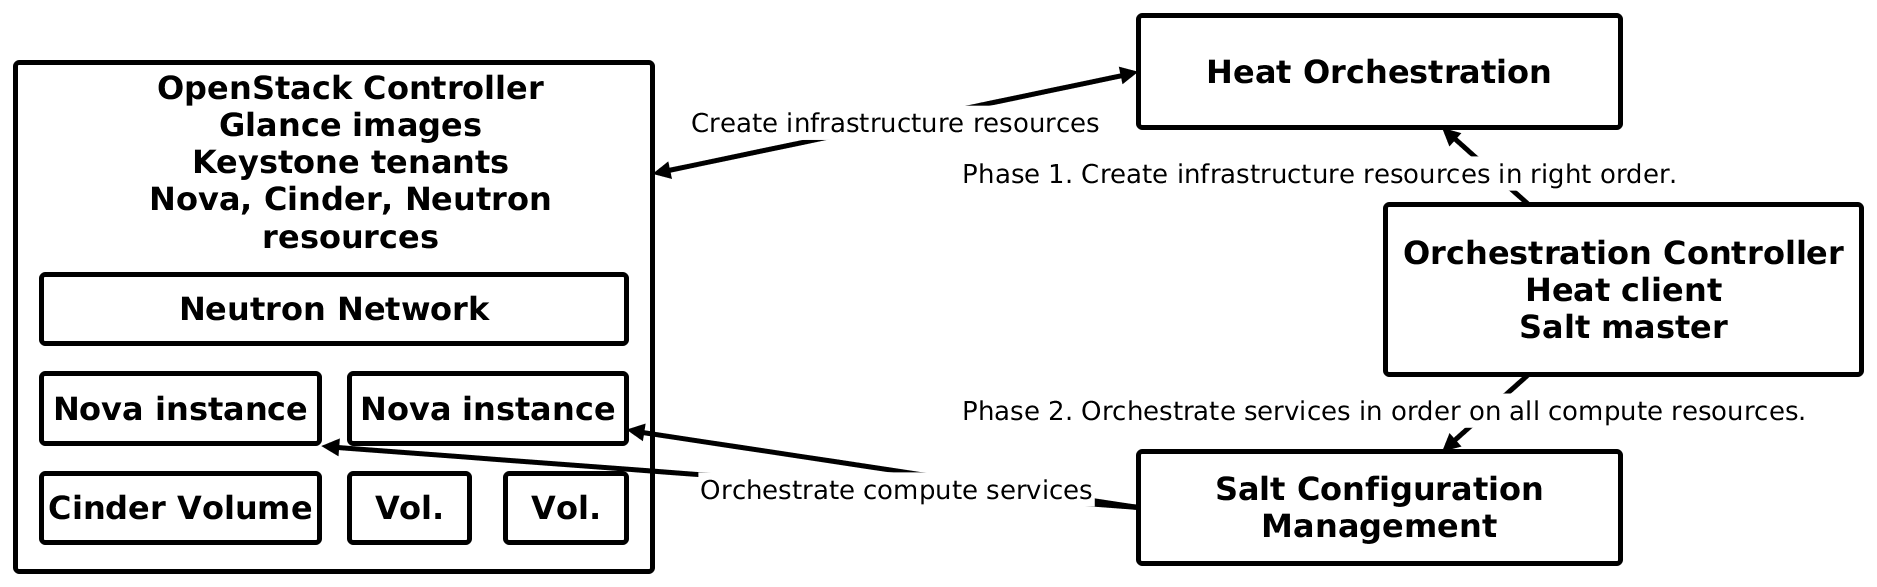
\includegraphics[scale=0.21]{images/heat}
\par\end{centering}
\caption{Popis heat orchestrace\label{fig:heat}}
\end{figure}

\section{Load balancer as a Service}

První VNF, která byla pro uživatele navržena, je Load balancing. 

 

\begin{figure}[h]
\begin{centering}
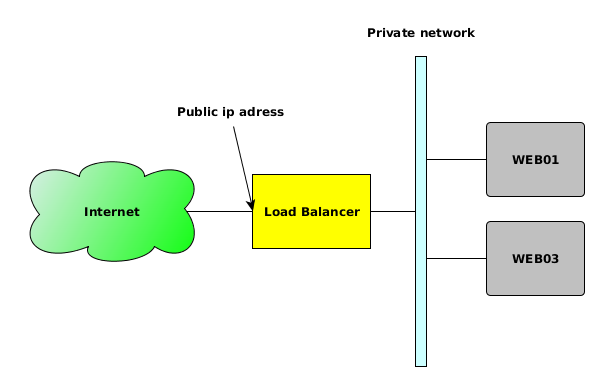
\includegraphics[scale=0.43]{images/LoadBalancer}
\par\end{centering}
\caption{Load Balancer as a Service\label{fig:LoadBalancer}}
\end{figure}

\subsection{Neutron LbaaS}

Součástí OpenStacku je Neutron HAproxy. 

Pro účely load balancingu byla použita existující implementace HAProxy Neutron LbaaS v OpenContrail.

Výhodou tohoto řešení je, že není nutná dodatečná kongigurace load balanceru. Vše co třeba je obsaženo v heat templatu.

\begin{figure}[h]
\begin{centering}
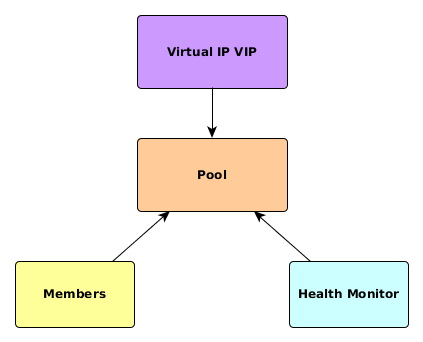
\includegraphics[scale=0.63]{images/NeutronLbaaS}
\par\end{centering}
\caption{Neutron LbaaS\label{fig:NeutronLbaaS}}
\end{figure}


\subsection{LbaaS template}

Navržený heat template pro LbaaS v sobě obsahuje následující prostředky, které se po spuštění pokusí vytvořit.

\begin{itemize}
\item pool
\item members
\item health monitoring
\item 2 web instance
\item privatni síť
\item public síť
\end{itemize}



\section{Firewall as a Service}

Servisní Template obsahuje obecný předpis pro danou VNF. Mezi tyto informace patří:

\begin{itemize}
\item Název - Název je označení daného Servisního Templatu. Pomocí něho lze následně identifikovat daný template a spustit dle jeho parametrů Servisní instanci. 
\item Image - Image je image, který má být použit pro vytvoření dané servisní instance. V našem případě se bude jednat o image, který obsahuje požadované síťové funkce. Tento image musí před tím než může být použit  nahrán do OpenStacku přes glance.
\item Service Type - V OpenContrailu, prozatím existují dva typy. Jsou to Trafic Analyzer a Firewall. Pro účely této práce bude používán pouze typ Firewall.
\item Service Mode - Zde se určuje v jakém modu daný template bude nastaven. Jsou zde možnosti In-Network, In-Network-NAT.

\item Typy síťových portů - Zde se určuje kolik portů bude daná instance, vytvořená pomocí tohoto templatu mít a jaká bude jejich role. Jsou zde možnosti Left, Right a Management. 

\end{itemize}

Po uspěšném vytvoření Servisního templatu je možné z něj vytvořit libovolný počet Servis Instancí. Ty běží jako klasické instance v OpenStacku, avšak OpenContrail s nimi zachází jiným způsobem. 

\begin{itemize}
\item 1 firewall instanci
\item 1 testovaci instanci
\item 1 management instanci
\item management síť
\item privátní síť
\item contrail policy
\end{itemize}

\subsection{Scénář NAT}


\begin{figure}[h]
\begin{centering}
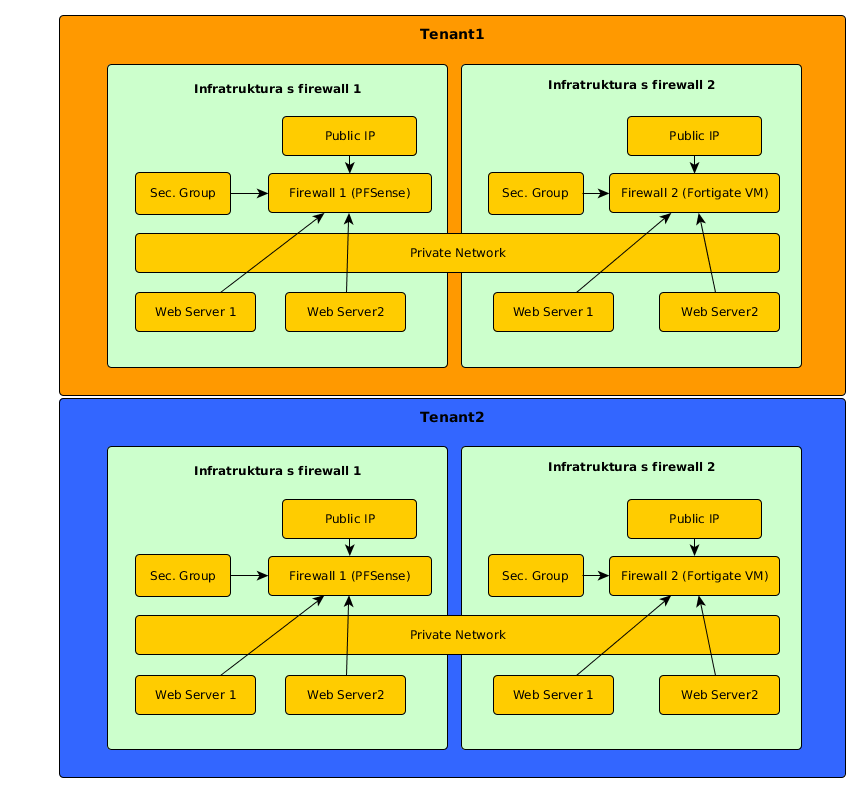
\includegraphics[scale=0.43]{images/firewall}
\par\end{centering}
\caption{Firewall as a Service\label{fig:firewall}}
\end{figure}

\subsection{Scénář HA firewall}

\begin{figure}[h]
\begin{centering}
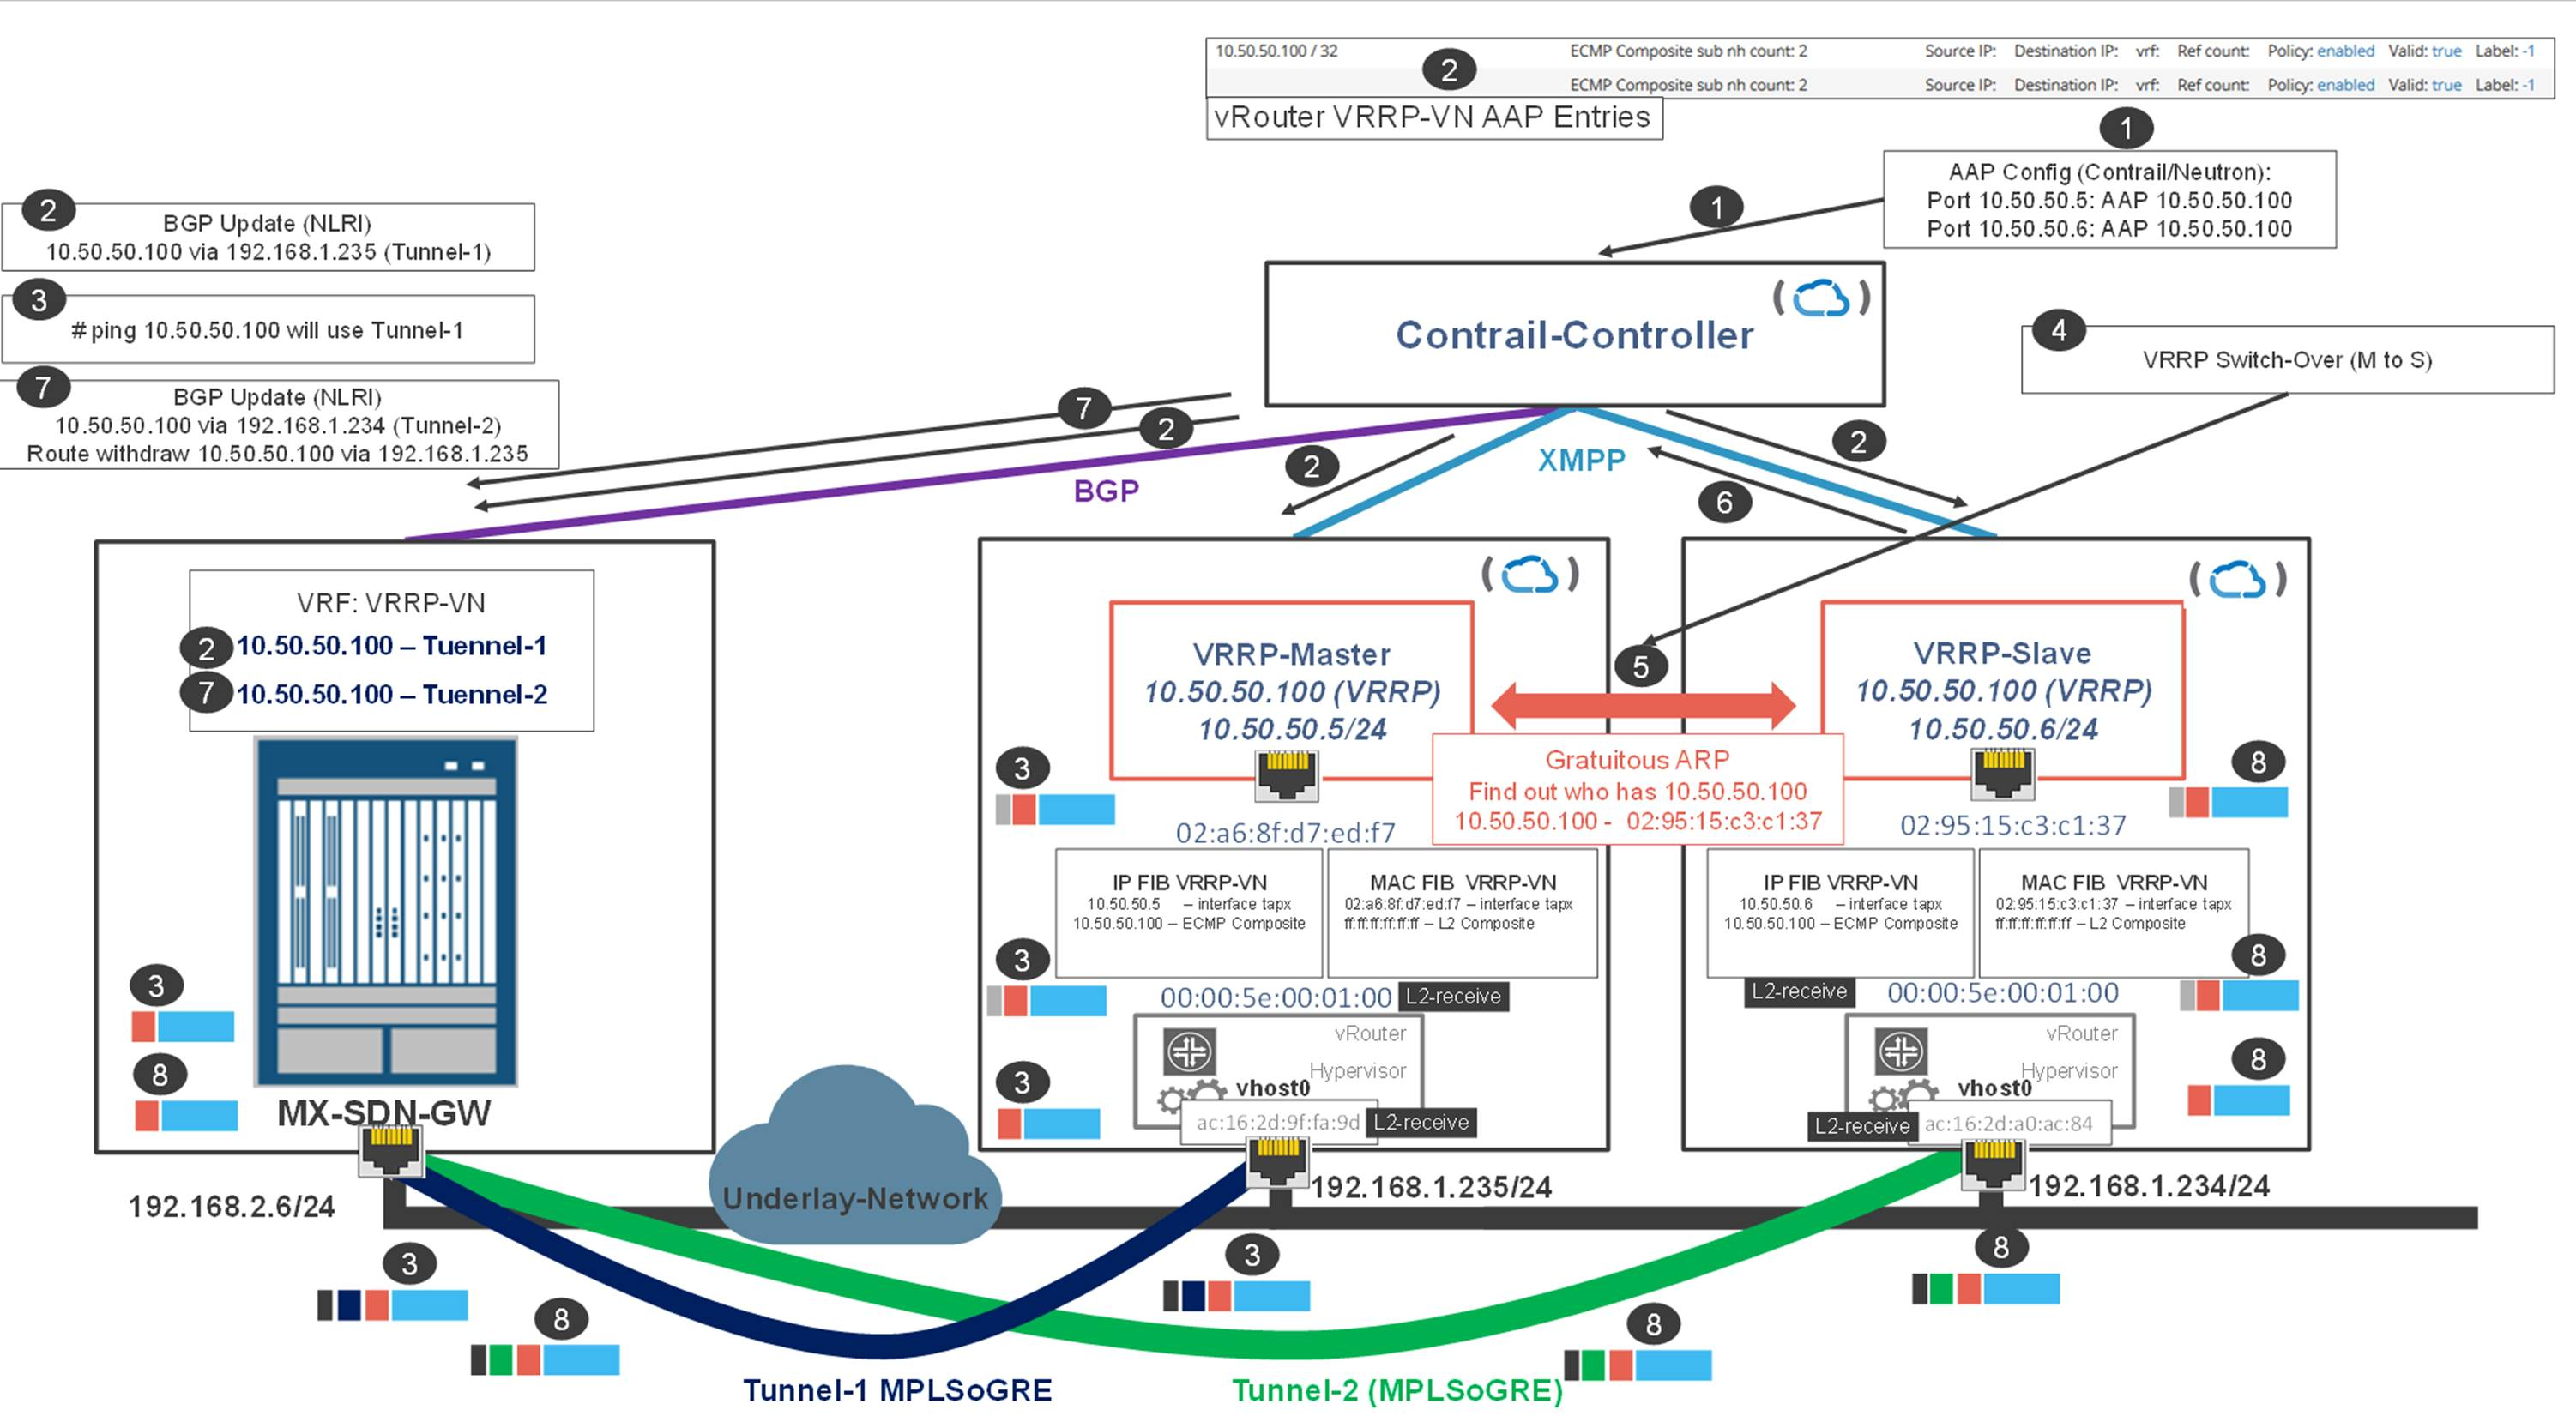
\includegraphics[scale=0.11]{images/contrailHA}
\par\end{centering}
\caption{High Availability Firewall\label{fig:contrailHA}}
\end{figure}


\subsection{FwaaS template}

Pro FwaaS je narhnut heat template, který obsahuje:





